In 1964 a catastrophic flood struck the city of Zagreb. Many buildings were completely destroyed when the water struck their walls. In this task, you are given a simplified model of the city before the flood and you should determine which of the walls are left intact after the flood.

The model consists of $N$ points in the coordinate plane and $W$ walls. Each wall connects a pair of points and does not go through any other points. The model has the following additional properties:

\begin{itemize}
\item No two walls intersect or overlap, but they may touch at endpoints;
\item Each wall is parallel to either the horizontal or the vertical coordinate axis.
\end{itemize}

Initially, the entire coordinate plane is dry. At time zero, water instantly floods the exterior (the space not bounded by walls). After exactly one hour, every wall with water on one side and air on the other breaks under the pressure of water. Water then floods the new area not bounded by any standing walls. Now, there may be new walls having water on one side and air on the other. After another hour, these walls also break down and
water floods further. This procedure repeats until water has flooded the entire area.

An example of the process is shown in the following figure.

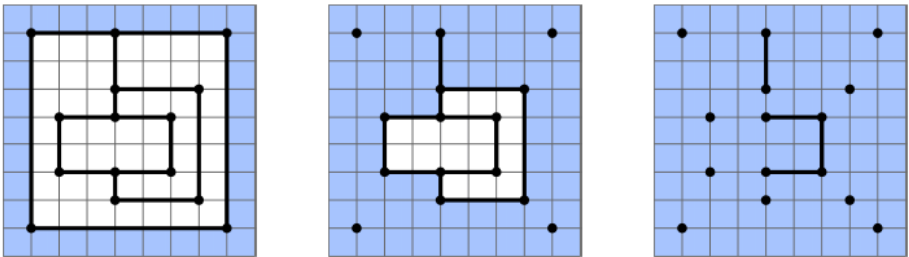
\includegraphics[scale=0.5]{flood.png}

The first picture shows the state at time zero. Shaded cells represent the flooded area, while white cells represent dry area (air). The second picture shows the state after one hour. The third picture shows state after two hours. Water has flooded the entire area, and the 4 remaining walls cannot be broken down.

Write a program that, given the coordinates of the $N$ points, and the descriptions of $W$ walls connecting these points, determines which of the walls are left standing after the flood.
